\documentclass{article}
  \usepackage[pdftex]{graphicx}
  \usepackage{pslatex}
  \usepackage{amsmath}
 \usepackage{amsfonts}
 \usepackage{textcomp}
\newtheorem{theorem}{Theorem}
\newenvironment{proof}[1][Proof]{\begin{trivlist}
\item[\hskip \labelsep {\bfseries #1}]}{\end{trivlist}}
\newenvironment{definition}[1][Definition]{\begin{trivlist}
\item[\hskip \labelsep {\bfseries #1}]}{\end{trivlist}}
\newenvironment{example}[1][Example]{\begin{trivlist}
\item[\hskip \labelsep {\bfseries #1}]}{\end{trivlist}}
\newenvironment{remark}[1][Remark]{\begin{trivlist}
\item[\hskip \labelsep {\bfseries #1}]}{\end{trivlist}}

%  \usepackage{qtree}

\begin{document}

\begin{center}
  \Large\bf
  Lecture Notes for Advanced Algorithms\\

  \medskip
  \large\sf
  Lecture of October 8, 2012\\
\end{center}

\section{Online Algorithms and Competitive Analysis}

Online algorithms are distinguished from offline algorithms by the following
features:
\begin{itemize}
\item They do not receive all of its input at once, 
but instead work on partial information
of requests $\sigma = \sigma(1) \sigma(2) \ldots \sigma(n)$. 
When the online algorithm is serving the request $\sigma(i)$, 
it has no information about the future requests $\sigma(i')$, where $i'>i$.
\item They work in a local/greedy fashion, only with the current moment and the past.
\item They are not always optimal; often because it is impossible to make global
assumption about the data, and the decisions that are made may turn out
to not be optimal in the future.
\end{itemize}

In order to analyze online algorithms, we deploy a technique called competitive analysis, 
where the performance is compared with the performance of an offline optimal algorithm. 
The formal definition of this is:
\begin{align}
  C_A &\leq kC_{opt} + O(1) \nonumber
\end{align}
We say an algorithm is k-competitive if its cost, $C_A$ is less or equal to the cost of the offline optimal algorithm, 
$C_{opt}$, multiplied by a positive constant $k$ and to which is added some constant. 
Competitive analysis is an amortized analysis, but, instead of proving something
absolute about the performance of the algorithm, it proves something relative: 
that the algorithm does not do worse than some constant times the performance of an optimal (usually unknown) strategy.


\section{Move-To-Front : Competitive Analysis}
We will run a competitive analysis of the Move-to-Front(MTF)
heuristic for list update problem.
\begin{figure}[h!]%
  \centering
    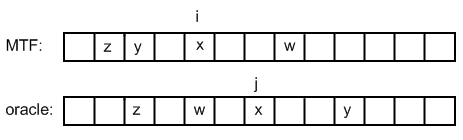
\includegraphics[scale = 0.5]{figures/figure1.png}%
  \caption{The general situation in the analysis of Move-To-Front.}%
  \label{fig:figure1}%
\end{figure}%
In Figure~\ref{fig:figure1}, the oracle list is the unknown optimal list.
The MTF list is maintained by moving the accessed element to the front of
the list.  As always, our potential function will quantify how poor our
current structure is.  In comparing our MTF list with the oracle list
on a query for $x$, we can partition the elements in front of $x$ in
the MTF list into two subsets: those that also occur in front of $x$
in the oracle list, and those that occur after $x$ in the oracle list.
The former are no problem: both the oracle and the MTF heuristic have
to pay one unit of actual running time for each such element; but the latter
cause the access to $x$ to run more slowly in the MTF list than in the
oracle list.  We will thus define the potential of $x$, $\phi(x)$, to
be the number of elements in this second category.
(Notice that we could consider the other side of the coin, namely elements
that occur before $x$ in the oracle list, but after $x$ in the MTF list,
and thus apparently yield an advantage to the MTF heuristic.  We do not
do it for two reasons: first, we are focused on the performance of MTF,
and that is determined entirely by the elements in front of $x$ in the MTFs
list; and secondly, because it is simpler and works!\ \ Naturally, we define
the potential of the MTF list as a whole as the sum of the potentials
of its elements, $\Phi=\sum_x\phi(x)$.

Assume $x$ is in the $i$th position in the MTF list.  The real cost of
accessing $x$ is then $i$; the real cost of moving $x$ to the front
of the list is constant---by keeping a pointer to the front of the list
and two pointers throughout the search (to the current and the previous
nodes on the list), we can move the node to the front in just three
pointer changes.  The change in potential due to moving $x$
to the front is then the sum of two contributions: $x$ will no longer
contribute anything to the potential (as it will no longer have
any elements in front of it), so we have a decrease of $\phi(x)$; but
all $i-1$ elements that were in front of $x$ now have an additional element
in front of them, $x$ itself, and thus their potential might be increased
by~$1$.  This increase only occurs if $x$, which is now in front of them
in the MTF list, is behind them in the oracle list---or, phrased in reverse,
the only elements affected are those that are in front of $x$ in the oracle
list.  We had partitioned
these $i-1$ elements earlier into two categories and counted $\phi(x)$
of them in the category of elements behind $x$ in the oracle list, so
there are $i-1-\phi(x)$ of them in front of $x$ in the oracle list.  Thus,
in addition to the decrease by $\phi(x)$ due to the loss of the direct
contribution of $x$, there is an increase by $i-1-\phi(x)$ due to the new
indirect contribution of $x$, for a total change of potential of
  $$-\phi(x) + (i-1-\phi(x) = i-1-2\phi(x)$$
Adding the real cost, we get, for a query to $x$ in the MTF list
  $$\text{real cost} + \Delta\Phi = 2\cdot (i-\phi(x))-1$$
Now we must turn to the cost and change in potential in the oracle list.

\subsection{Oracle: Static Version}
\label{sec;static}
We begin with the static version of the oracle: the list of the oracle
will never be changed---it is read-only. Therefore, there is no change
in the potential due the oracle itself.  The real cost of the oracle
is simply $j$, the index of the query element $x$ in the oracle list.

To compare the oracle ($j$) with MTF ($2\cdot(i-\phi(x))-1$),
examine Figure~\ref{fig:figure2}.
\begin{figure}[h!]%
  \centering
    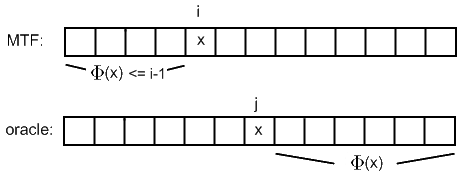
\includegraphics[scale = 0.5]{figures/figure2.png}%
  \caption{Static version of the oracle---first look.}%
  \label{fig:figure2}%
\end{figure}%
We know that there are at least $\phi(x)$ elements behind $x$ in the oracle
list; we also know that there are exactly $j-1$ elements in front of $x$
in the oracle list and that the list has length~$n$.  Thus we can write
  $$(j-1)+1+\phi(x)\leq n$$
(The one is for $x$ itself.)\ \ Thus we can bound $j$ by $j\leq n-\phi(x)$.
But that is not the kind of bound we need: we need a lower bound for $j$,
not an upper bound.  We observed earlier that there are $i-1-\phi(x)$
elements that are in front of $x$ in \emph{both} lists: this gives us
the desired lower bound: these elements are among the $j-1$ in front
of $x$ in the oracle list, as illustrated in Figure~\ref{fig:figure3},
\begin{figure}[h!]%
  \centering
    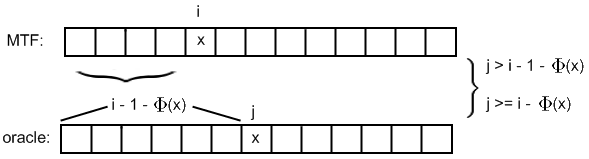
\includegraphics[scale = 0.5]{figures/figure3.png}%
  \caption{Static version of the oracle---second look.}%
  \label{fig:figure3}%
\end{figure}%
and thus we have
  $$j-1\geq i-1-\phi(x)$$
or, simplifying
  $$j\geq i-\phi(x)$$
But now we can go back to the MTF amortized cost
  $$\text{real cost} + \Delta\Phi = 2\cdot (i-\phi(x))-1 \leq 2j -1 < 2j$$
and we have shown that the amortized cost of the MTF list is strictly less
than twice that of the optimal static list.

\subsection{Oracle (Optimal) : Dynamic Version}
\label{sec;dynamic}
Obviously, the all-knowing oracle can do better if it restructures its list
between accesses.  We need to look at the kind of moves it can make.
First, it can move $x$ itself, either towards the front or towards the back.
Secondly, it can move any other elements it chooses, again towards the front
or towards the back.  The oracle must pay for moves deeper into the list
(towards the back), but moves towards the front are free---it can keep
a pointer to the node in front of the place where it wants to move $x$.
Additional real costs for the oracle go on the right-hand side of the
inequality and so can only help us; potential changes go on the left-hand
side, so that decreases in potential can only help, while increases in
potential could damage the inequality unless they can be suitably bounded.

Let us start with moving only $x$.  If the oracle decides to move $x$
towards the back, say by $k$ positions, it will incur an added cost of $k$,
which goes on the right-hand side of the inequality we want to maintain.
But it will also alter the potential, and the potential change goes on
the left-hand side of the inequality, as part of our amortization.
What is that change in potential?\ \ Well the potential of $x$ itself
can only decrease by such a move: there will be fewer elements behind it
in the oracle list---some of the $k-1$ elements between the original and
new positions of $x$ could be in front of $x$ in the MTF list,
as illustrated in Figure~\ref{fig:figure4}.
\begin{figure}[h!]%
  \centering
    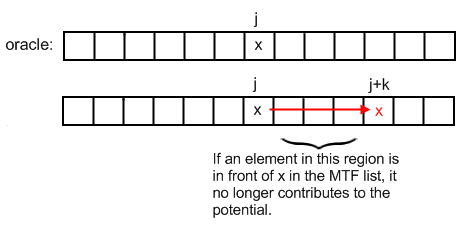
\includegraphics[scale = 0.5]{figures/figure4.png}%
  \caption{Dynamic version of the oracle: $x$ is moved towards the back.}%
  \label{fig:figure4}%
\end{figure}%
The contribution $\phi(z)$ of an element $z$ that was on front of $x$ in
the oracle list is not affected by this move, nor is the contribution
$\phi(y)$ of an element $y$ that is behind the new position of $x$ in
the oracle list---in both cases, the sets of elements in front of,
and behind $z$, or $y$, have not changed.  Finally, the contribution $\phi(w)$
of an element $w$ that is between the original and the new positions
of $x$ in the oracle list can increase by one, if $x$ is in front
of $w$ in the MTF list.  In summary, the change in potential is limited
to two parts: those of the $k-1$ elements between the old and the new positions
of $x$ in the oracle list that are in front of $x$ in the MTF list
will cause a decrease of one unit each in $\phi(x)$, and the others
will see an increase of one unit each in their own $\phi$ contribution.
There is no way for us to know how many elements are in each of these
two categories, but it does not matter: the change of potential must be
in the range
  $$[-(k-1),\ldots,0,\ldots,k-1]$$
and so is always less than
the added real cost.  Thus, if the oracle moves element $x$ to the back,
the inequality is maintained.

Let us then look at the case where the oracle moves $x$ towards the front,
illustrated in Figure~\ref{fig:figure5}.
\begin{figure}[h!]%
  \centering
    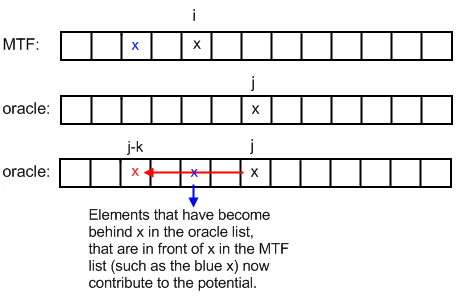
\includegraphics[scale = 0.5]{figures/figure5.png}%
  \caption{Dynamic version of the oracle: $x$ is moved towards the front.}%
  \label{fig:figure5}%
\end{figure}%
In this case, we are not interested in elements that are in front of $x$ in the
MTF list and behind $x$ in the oracle list, since their positions will remain
the same relative to $x$, even after $x$ is moved up in the oracle list.
In this case also, the real cost to the oracle does not increase: it remains
just~$j$.
The elements of interest are again those between the new and the old positions
of $x$ in the oracle list.  Among these elements, those that are in front of
$x$ in the MTF list (the blue elements in the figure) will each add one unit
to the potential of $x$; we can bound the number of such elements by
$\min(k-1, i-1-\phi(x))$.
Those that are behind $x$ in the MTF list will each see their potential
decrease by one unit, as $x$ was one of the elements in front of them
in the MTF list, but behind them in the oracle list, but is now in front
of them in both lists.  As in the analysis of a move towards the back,
we cannot determine how many of the $k-1$ elements fall into each of
these two categories, but we can state that the combined change in potential
must be in the range
  $$[-(k-1),\ldots,0,\ldots,\min\{k-1,i-1-\phi(x)\}]$$
Hence, in the worst case, the left-hand side of the inequality goes up by
$i-1-\phi(x)$, which is less than $j$, and so we can maintain the inequality
simply by using a ratio of 3 instead of 2.  (By using a slightly more
elaborate potential and incorporating elements that occur before $x$ in the oracle list but after $x$ in the MTF list, 
we can in fact keep the 2.)

In order to complete the analysis, we need to verify that the inequality
(perhaps again with a higher ratio) remains satisfied if the oracle moves
elements other than $x$ itself.  The reasoning remains similar to the above,
but the cases multiply (for instance, a move towards the back is free
if the element moved stays in front of the old position of $x$, but
moving more than one element may incur additional costs---we have to keep in
mind that the structure being manipulated is a linked list and the oracle
is bound by the same operations as any algorithm).  We leave the rather
tedious details to the reader, but note that, with the slightly
more elaborate line of reasoning alluded to in the previous paragraph,
we can keep a ratio of 2.

As a remark, the beauty of competitive analysis is that it enables
us to compare an algorithm to an optimal strategy, despite the fact
that this optimal strategy is unknown.

\section{Paging Algorithms}
\label{sec:PA}
We assume a two-level memory system, cache and main memory.
When CPU executes sequence of operations $\sigma = \sigma(1) \sigma(2) \ldots \sigma(n)$,
it reads data from the cache. Cache memory access is very fast, but it has very limited capacity.
The main memory has larger capacity, but the access of the main memory is much slower.
When operation $\sigma(i)$ is asking for certain page,
the processor looks for required page in the cache. 
If it is not found, there is a \emph{page fault} event. 
Missing page has to be brought into the cache from the main memory, which is of high capacity, but slow access.


In order to maximize efficiency we need to minimize number of page faults.
Many cache algorithms has been developed for this purpose. If processor needs
new page, but cache is full, they decide which page should be discarded. Examples:


\begin{itemize}
  \item FIFO (First In First Out): In this strategy, we remove the old-
est page from the cache. The assumption is that old page finished its job, so
it will not be used in a future. Bad side of this approach is that page will be
deleted even if it is used frequently, only because of its age.
  \item LRU (Least Recently Used): We choose the least recently used
page to be discarded. If some page was required in the close past, probably we
will use it again soon.
  \item LFU (Least Frequently Used): We choose the page which is
used the least number of times. On page fault we throw out the page with lowest
counter value. Disadvantage of this strategy is that old pages are privileged
because counter of the new one starts with 0.
\end{itemize}

\textbf We will illustrate the performance of the above algorithms on the following example, 
with cache size $k = 3$ and input set $\sigma = 23123412$.
\begin{center}
 \begin{tabular} {|c|c|c|c|c|c|c|c|c|}
\hline
$\sigma$ & 2  & 3 & 1 & 2 & 3 & 4 & 1 & 2 \\
\hline
 FIFO & $\times$ & $\times$ & $\times$ & $\checkmark$ & $\checkmark$ & $\times$ & $\checkmark$ & $\times$ \\
\hline
 LRU & $\times$ & $\times$  & $\times$  & $\checkmark$ & $\checkmark$ & $\times$ & $\times$ & $\times$ \\
\hline
 LFU & $\times$  & $\times$  & $\times$  & $\checkmark$ & $\checkmark$ & $\times$ & $\times$ & $\checkmark$ \\
\hline
\end{tabular}
\end{center}

\begin{itemize}
\item OPT (Optimal Offline Paging Algorithm): Discard the page for which the next
request occurs the latest in a future.
\end{itemize}
\begin{center}
 \begin{tabular} {|c|c|c|c|c|c|c|c|c|}
\hline
$\sigma$  & 2  & 3 & 1 & 2 & 3 & 4 & 1 & 2 \\
\hline
 OPT & $\times$ & $\times$ & $\times$ & $\checkmark$ & $\checkmark$ & $\times$ & $\checkmark$ & $\checkmark$ \\
\hline
\end{tabular}
\end{center}


%\subsection{Competitive analysis of LFU strategy for page replacement}
\begin{theorem}
LFU is not $c$-competitive for any constant $c$.
\end{theorem}
\begin{proof}
In order to demonstrate that LFU is not $c$-competitive for any constant $c$, 
we need to find a request sequence such that, the ratio between $C_{LFU}(\sigma)$ and $C_{OPT}(\sigma)$ 
can be arbitrarily large.\\
Let $\sigma=\overbrace{1 1\cdots 1}^{m \text{ times}}\overbrace{2 2\cdots 2}^{m \text{ times}} \cdots 
\overbrace{k k\cdots k}^{m \text{ times}} \overbrace{(k+1)(k+2) (k+1)(k+2)\cdots (k+1)(k+2)}^{m \text{ times}}$, 
where $k$ is the cache size. 
Then $C_{LFU}(Q) = k + 2m$ and $C_{OPT}(Q) = k + 2$. 
Since we can choose any $m$, 
there exist no constant $c$ such that $k + 2m \leq c(k + 2) + a$. 
Therefore, the LFU strategy is not $c$-competitive for any constant $c$.
\end{proof}

%\subsection{Competitive analysis of FIFO and LRU strategy for page replacement}
\begin{theorem}
FIFO and LRU are $k$-competitive where $k$ is the cache size.
\end{theorem}

We would like to get an upper bound cost of FIFO and LRU and a lower bound of OPT. 
In order to find the desired lower and upper bounds, we recursively define \emph{phases}. 
Phase $0$ consists of the first $k$ distinct pages in the request sequence. 
Phase $i + 1$ starts from the first page which is distinct with respect to phase $i$ and contains the next $k$ distinct pages. 
An example for $k=3$ and the request sequence $\sigma$:

\begin{align*}
  \sigma = \overbrace{2 3 4}^{\text{Phase 0}} \overbrace{1 2 3 2 1}^{\text{Phase 1}} \overbrace{4 4 2 4 4 3}^{\text{Phase 2}} \overbrace{1 3 4 3}^{\text{Phase 3}}
\end{align*}.

We can verify that the following lower and upper bounds:
\begin{align*}
   C_{FIFO}, C_{LRU} &\leq k \times number~of~phases \\
  C_{OPT} &\geq number~of~phases
\end{align*}
In sum, we have $C_{FIFO}, C_{LRU} \leq k \times C_{OPT}$.

Competitive analyses show that the relative performances of FIFO and LRU are the same, which are better than that of LFU.
But LRU achieves much better performance than FIFO in real systems. 
The discrepancy between theory and practice reflects that one drawback of competitive analysis is 
that it always assumes a malicious adversary and may ignore useful distribution information of online requests. 
To improve the theoretical analysis, we can design more elaborate models, 
or deploy average-case analysis under reasonable assumptions. 
\end{document}
